\subsection{Synthetic Field Testing for the Enstrophy Transport Terms}
The following section describes the testing for the enstrophy transport
terms. The following velocity, vorticity, and subgrid stress fields were
used for testing
\begin{subequations}
    \begin{equation}
        u_{i} =  (x^2 y z, x y^2 z, x y z^2)
    \end{equation}
    \begin{equation}
        \omega_{i} =  (yz\sin x, xz\sin y, xy\sin z)
    \end{equation}
    \begin{equation}
        \tau_{ij} =
        \begin{pmatrix}
            x^2         & xy      &   xz  \\
            xy          & y^2     &   yz  \\
            xz          & yz      &   z^2  \\
        \end{pmatrix}
    \end{equation}
\end{subequations}
Calculating the $S_{ij}$ and $\Psi_{ij}$ from the velocity and subgrid
stress gives
\begin{subequations}
    \begin{equation}
        S_{ij} = 
        \begin{pmatrix}
            2xyz                                        &   \frac{1}{2}z\left(x^{2} + y^{2} \right)     &       \frac{1}{2}y\left(x^{2} + z^{2} \right)     \\
            \frac{1}{2}z\left(x^{2} + y^{2} \right)     &   2xyz                                        &       \frac{1}{2}x\left(y^{2} + z^{2} \right)     \\
            \frac{1}{2}y\left(x^{2} + z^{2} \right)     &   \frac{1}{2}x\left(y^{2} + z^{2} \right)     &       2xyz                                        \\
        \end{pmatrix}
    \end{equation}
    \begin{equation}
        \Psi_{ij} = 
        \begin{pmatrix}
            0           &       z       &           -y      \\
            -z          &       0       &           x       \\
            y           &       -x      &           0       \\
        \end{pmatrix}
    \end{equation}
\end{subequations}
\subsubsection{Results}
The following results below are for the testing of the enstrophy transport
terms.
\paragraph{A term}
\begin{figure}[H]
    \includegraphics[height=0.4\textheight]{media/enstrophy-transport-terms/A-term-approx.pdf}
    \caption{Approximate solution for $\aenst$ term}
    \label{fig:a-approx}
\end{figure}
\begin{figure}[H]
    \includegraphics[height=0.4\textheight]{media/enstrophy-transport-terms/A-term-exact.pdf}
    \caption{Exact solution for $\aenst$ term}
    \label{fig:a-exact}
\end{figure}
\paragraph{B term}
\begin{figure}[H]
    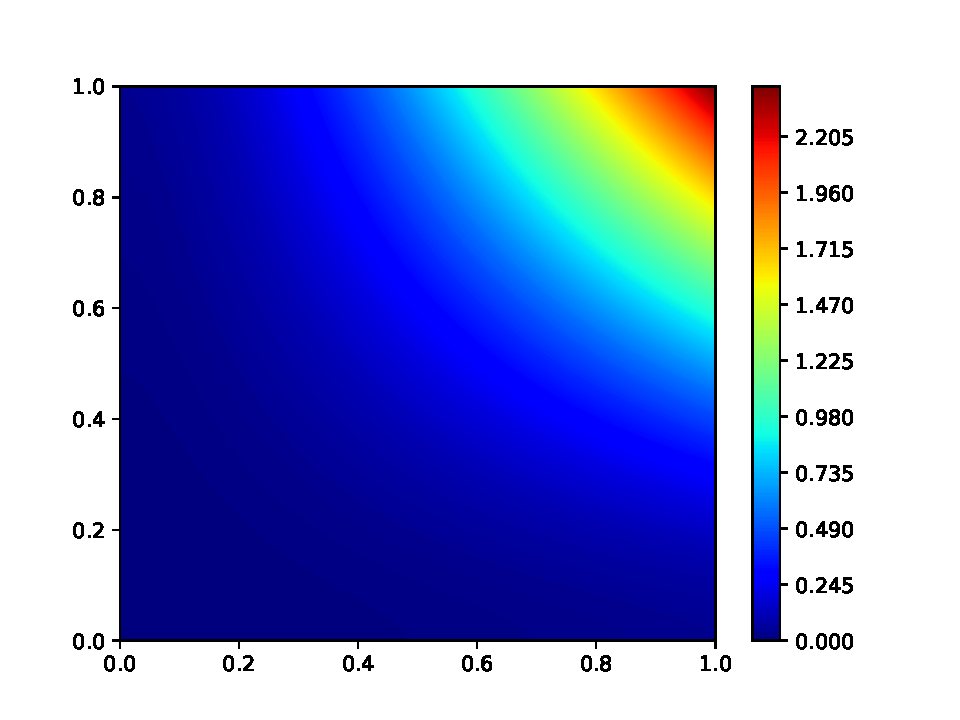
\includegraphics[height=0.4\textheight]{media/enstrophy-transport-terms/C-term-approx.pdf}
    \caption{Approximate solution for $\benst$ term}
    \label{fig:b-approx}
\end{figure}
\begin{figure}[H]
    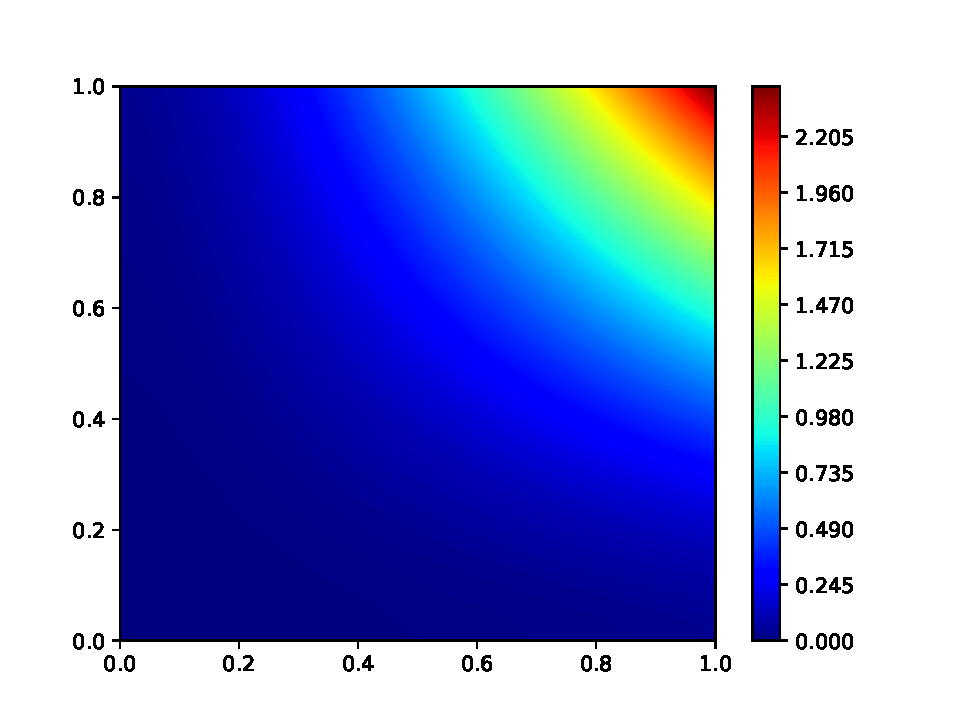
\includegraphics[height=0.4\textheight]{media/enstrophy-transport-terms/C-term-exact.pdf}
    \caption{Exact solution for $\benst$ term}
    \label{fig:b-exact}
\end{figure}
\paragraph{D term}
\begin{figure}[H]
    \includegraphics[height=0.4\textheight]{media/enstrophy-transport-terms/D-term-approx.pdf}
    \caption{Approximate solution for $\denst$ term}
    \label{fig:d-approx}
\end{figure}
\begin{figure}[H]
    \includegraphics[height=0.4\textheight]{media/enstrophy-transport-terms/D-term-exact.pdf}
    \caption{Exact solution for $\denst$ term}
    \label{fig:d-exact}
\end{figure}
\begin{figure}[H]
    \includegraphics[height=0.4\textheight]{media/enstrophy-transport-terms/SGS-trans-approx.pdf}
    \caption{Approximate solution for $\pienst$ term}
    \label{fig:pi-approx}
\end{figure}
\begin{figure}[H]
    \includegraphics[height=0.4\textheight]{media/enstrophy-transport-terms/SGS-trans-exact.pdf}
    \caption{Exact solution for $\pienst$ term}
    \label{fig:pi-exact}
\end{figure}
\begin{figure}[H]
    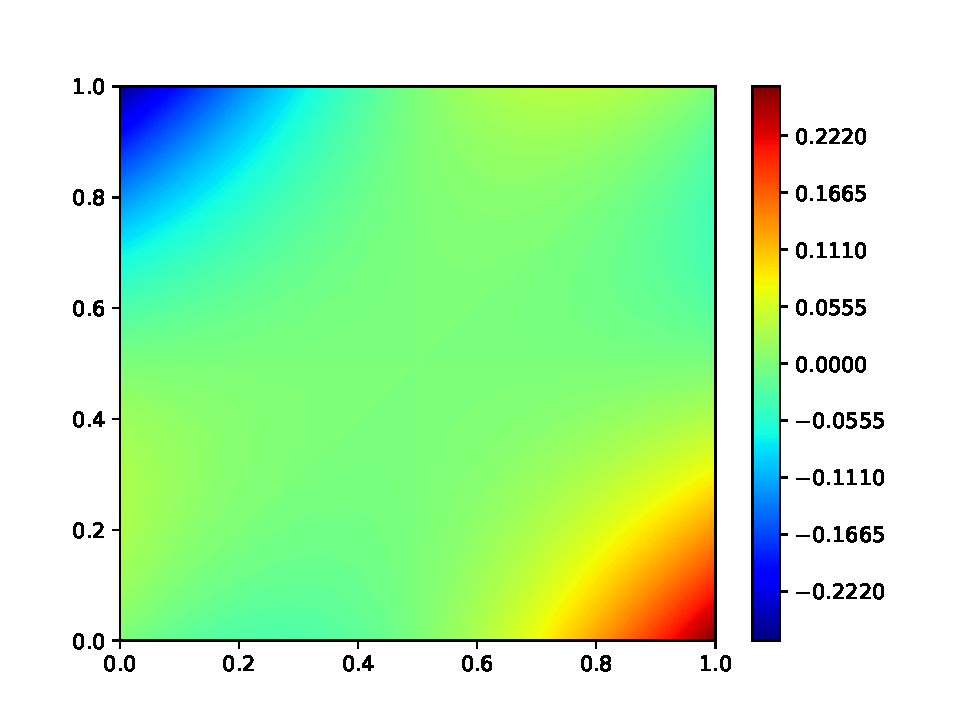
\includegraphics[height=0.4\textheight]{media/enstrophy-transport-terms/SGS-prod-approx.pdf}
    \caption{Approximate solution for $\penst$ term}
    \label{fig:p-approx}
\end{figure}
\begin{figure}[H]
    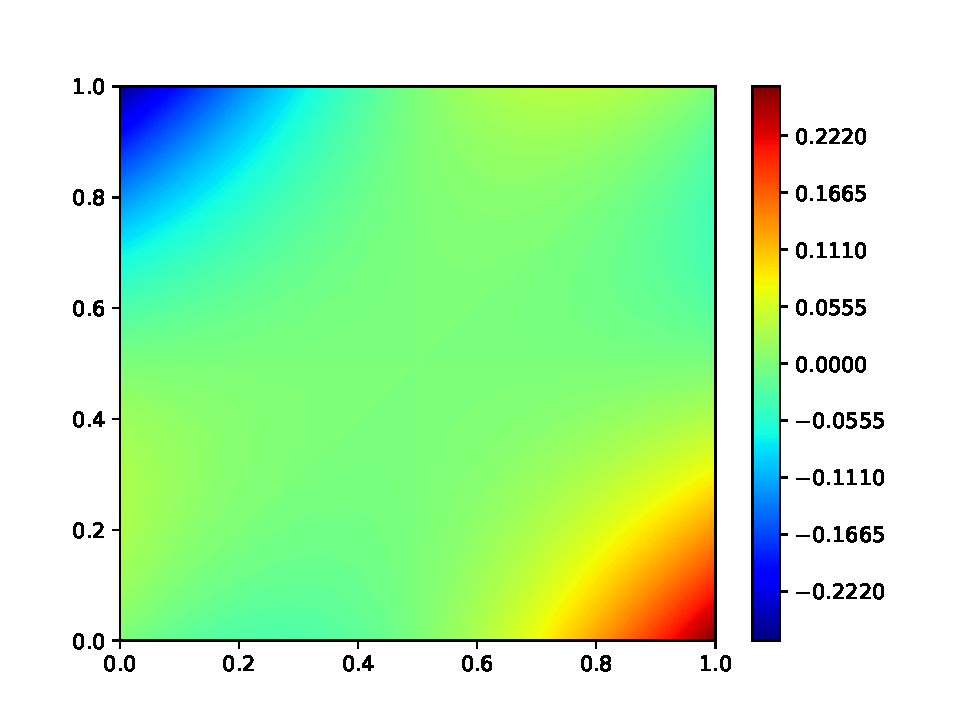
\includegraphics[height=0.4\textheight]{media/enstrophy-transport-terms/SGS-prod-exact.pdf}
    \caption{Exact solution for $\penst$ term}
    \label{fig:p-exact}
\end{figure}
